\chapter{Aplicação de Monitoramento}
\label{chap4}

Após o detalhamento da arquitetura e dos componentes do sistema de monitoramento, este capítulo apresenta a aplicação prática da solução desenvolvida. São abordados os dois mecanismos principais responsáveis pela visualização e notificação das métricas coletadas: o dashboard e o sistema de alertas.

Na primeira seção, é detalhado o dashboard implementado, incluindo os gráficos e visualizações criados, os códigos PromQL utilizados nas consultas correspondentes e os procedimentos de processamento dos dados. A segunda seção descreve o sistema de alertas, abrangendo as regras de disparo de notificações, a configuração dos pontos e canais de contato, bem como a experiência prática obtida com os diferentes sistemas de alertas disponíveis no ecossistema adotado. A terceira seção apresenta um caso de uso prático, ilustrando a aplicação do sistema de monitoramento em um cenário real.

\section{Dashboard}
\label{section:Dashboard}

Conforme mencionado ao longo deste trabalho, os princípios de IaC são fundamentais para assegurar a reprodutibilidade e o versionamento de toda a infraestrutura desenvolvida. Essa abordagem abrange não apenas os componentes centrais do projeto, mas também os dashboards e sistemas de alertas configurados. Por meio de arquivos declarativos YAML, são definidas e versionadas as configurações internas, o processamento de dados, as consultas PromQL e as regras de alertas (conforme será detalhado na Seção \ref{section:Alertas}), automatizando integralmente o fluxo de trabalho.

A configuração do Prometheus como fonte de dados padrão do Grafana foi realizada através do arquivo \verb|datasource.yaml|, enquanto as configurações internas específicas do dashboard foram estabelecidas no arquivo \verb|dashboards.yml|, conforme apresentado nos Códigos Fonte \ref{lst:default-datasource} e \ref{lst:dashboards-yml}, respectivamente.

\begin{lstlisting}[caption={Arquivo datasource.yml}, label={lst:default-datasource}]
apiVersion: 1
datasources:
- name: Prometheus
  type: prometheus
  access: proxy
  url: http://prometheus:9090
  isDefault: true
\end{lstlisting}

\begin{lstlisting}[caption={Arquivo dashboards.yml}, label={lst:dashboards-yml}]
apiVersion: 1
providers:
  - name: 'monitoring'
    orgId: 1
    folder: 'Monitoring'
    type: file
    disableDeletion: false
    updateIntervalSeconds: 5
    options:
      path: /etc/grafana/dashboards
      foldersFromFilesStructure: false
\end{lstlisting}

Para o processamento dos dados, adotou-se uma abordagem híbrida: a normalização dos dados foi implementada por meio de consultas PromQL estruturadas em arquivos YAML e executadas como \verb|Recording Rules| diretamente no Prometheus, enquanto as consultas específicas de cada gráfico foram definidas na interface web do Grafana.

O cenário ótimo consistiria na utilização exclusiva de \texttt{Recording Rules} para todo o processamento de dados, uma vez que as consultas PromQL executadas pelo Grafana seguem o fluxo: Grafana \foreign{frontend} $\rightarrow$ Grafana \foreign{backend} $\rightarrow$ Prometheus, retornando subsequentemente pelos mesmos componentes em ordem inversa para entregar os resultados de cada consulta. Em contrapartida, as \verb|Recording Rules| realizam o processamento internamente no Prometheus (exemplo de benefício do TSDB), otimizando o desempenho.

Embora computacionalmente mais eficientes, as \texttt{Recording Rules} apresentam limitações operacionais como a incompatibilidade com as variáveis dinâmicas do Grafana (\verb|Grafana Variables|) e a necessidade de reinicialização do Prometheus para aplicar modificações nas regras. Diante destas restrições, a abordagem híbrida oferece maior praticidade e conveniência para o desenvolvimento de dashboards, ainda que implique em um custo computacional superior.

Na normalização dos dados no Prometheus, são realizadas duas operações principais, quando aplicáveis: a conversão de métricas com diferentes unidades (como microssegundos, bytes, contagens) para formatos padronizados, como percentuais; e a transformação de métricas provenientes de diferentes hosts para um formato consistente, possibilitando comparações e visualizações agregadas.

Um exemplo prático dessa normalização é a métrica de uso de CPU "Carga de usuário" no host físico, ela representa uma porcentagem de utilização por tempo total, enquanto nos dispositivos virtuais é expressa como um valor acumulado em microssegundos desde a inicialização do contêiner correspondente. Para unificar essas métricas, utiliza-se a consulta PromQL apresentada no Código Fonte \ref{lst:cpu_user_load}. Além disso, esta normalização incluiu a padronização e otimização de labels, e a unificação das métricas numa única métrica consolidada: \verb|cpu_user_load|.

As funções \verb|label_replace| são empregadas para manipular as labels, enquanto a função \verb|irate| calcula a taxa de variação das duas amostras mais recentes da janela de tempo definida --- neste caso, 30 segundos, conforme a frequência de Nyquist. Essa taxa é convertida de microssegundos para segundos por meio da divisão por $10^{6}$ e, em seguida, multiplicada por 100 para obter o valor em percentual.

A métrica final \verb|cpu_user_load| é, então, utilizada nos gráficos do Grafana, oferecendo uma visão integrada do uso de CPU tanto para hosts físicos quanto para contêineres.

A escolha da função \verb|irate|, que calcula a taxa instantânea de variação, em detrimento da função \verb|rate|, que calcula a taxa média ao longo do intervalo, deve-se à necessidade de detectar variações rápidas, como picos de uso de CPU, que poderiam ser suavizados pela média.

\begin{lstlisting}[caption={Arquivo cpu.yml}, label={lst:cpu_user_load}]
groups:
  - name: cpu_normalization
    rules:
      - record: cpu_user_load
        expr: >
          label_replace(
            label_replace(
              irate(container_cgroup_cpu_stat_user_usec
              {job="virtual_hosts"}[30s]) 
              / 1e6 * 100,
              "instance", "", "", ""
            ),
            "path", "", "", ""
          )
        labels:
          unit: percent
      [...]
      - record: cpu_user_load
        expr: >
          label_replace(
            label_replace(
              physical_cpu_usage_user{job="physical_host"},
              "instance", "", "", ""
            ),
            "cpu", "", "", ""
          )
        labels:
          unit: percent
\end{lstlisting}

\newpage

\begin{lstlisting}[caption={Métricas de CPU \myenquote{Carga de usuário} pré-normalização}, label={lst:telegraf-cpu-user-load}]
  physical_cpu_usage_user{alias="Host Machine", cpu="cpu-total", host="6RW9K03", instance="172.17.0.1:9273", job="physical_host"}	16.283422459908643

  container_cgroup_cpu_stat_user_usec{alias="Ubuntu 1", host="device1", instance="device_1:9273", job="virtual_hosts", path="/sys/fs/cgroup/"}
     32102389
\end{lstlisting}

\begin{lstlisting}[caption={Métricas de CPU \myenquote{Carga de usuário} normalizadas}, label={lst:normalized-cpu-user-load}]
  cpu_user_load{alias="Host Machine", host="6RW9K03", job="physical_host", unit="percent"}	5.620946432860638 
  cpu_user_load{alias="Ubuntu 1", host="device1", job="virtual_hosts", unit="percent"}	
     0.59546
\end{lstlisting}

O restante dos arquivos de \verb|Recording Rules| do Prometheus podem ser encontrados no repositório do projeto \citep{vitorcossetti2025}, na pasta \verb|configs/prometheus/rules|.

Seguindo a abordagem híbrida e após o processamento dos dados no Prometheus, inicia-se a construção dos dashboards por meio da interface web do Grafana. Inicialmente, são criadas as \verb|Grafana Variables|, que atuam como filtros globais para todos os gráficos, permitindo a seleção dinâmica de parâmetros para uma visualização e interpretação mais eficientes dos dados. As variáveis configuradas estão listadas na Tabela \ref{tab:grafana-variables}:

\begin{table}[H]
\centering
\caption{Grafana Variables.}
\label{tab:grafana-variables}
\begin{tabular}{cl}
\toprule
\textbf{Variável} & \textbf{Filtro aplicado} \\
\midrule
\verb|Job| & Categoria do dispositivo (físico ou virtual) \\
\verb|Device| & Dispositivo (nome do host físico ou virtual) \\
\verb|Disk Partition| & Partição de disco (exemplo: \verb|/dev/sda1|) \\
\verb|Network Interface| & Interface de rede (exemplo: \verb|eth0|, \verb|wlan0|) \\
\bottomrule
\end{tabular}
\end{table}

Outra configuração global relevante refere-se aos intervalos de atualização e tempo aplicados a todos os gráficos. O intervalo de atualização define a frequência com que os dados são atualizados, enquanto o período temporal especifica o intervalo de tempo exibido nos gráficos. Embora esses parâmetros possam ser ajustados conforme a necessidade do usuário, para garantir um monitoramento próximo ao tempo real e sincronizado com as configurações de scraping do Telegraf e do Prometheus, o intervalo de atualização foi definido para 5 segundos e o período temporal para 5 minutos. Adicionalmente, tais valores podem ser modificados individualmente para cada gráfico, sendo que as configurações específicas prevalecem sobre as globais.

\begin{figure}[ht]
\centering
\setlength{\abovecaptionskip}{-20pt}
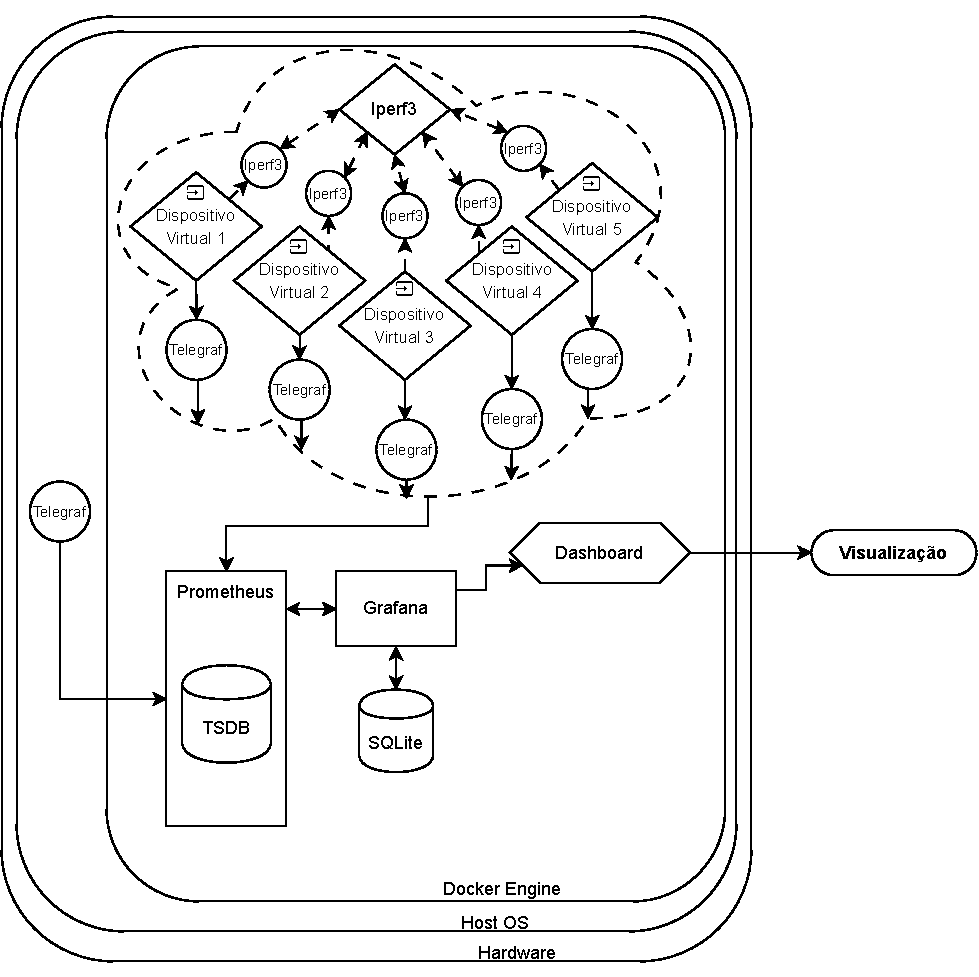
\includegraphics[width=\textwidth]{Imagens/chap04/by-blocks/dashboard_diagram.pdf}
\caption{Visualização.}
\label{fig:DiagramaVisualizacao}
\end{figure}

\begin{figure}[H]
\centering
\color{red}
\setlength{\abovecaptionskip}{-20pt}
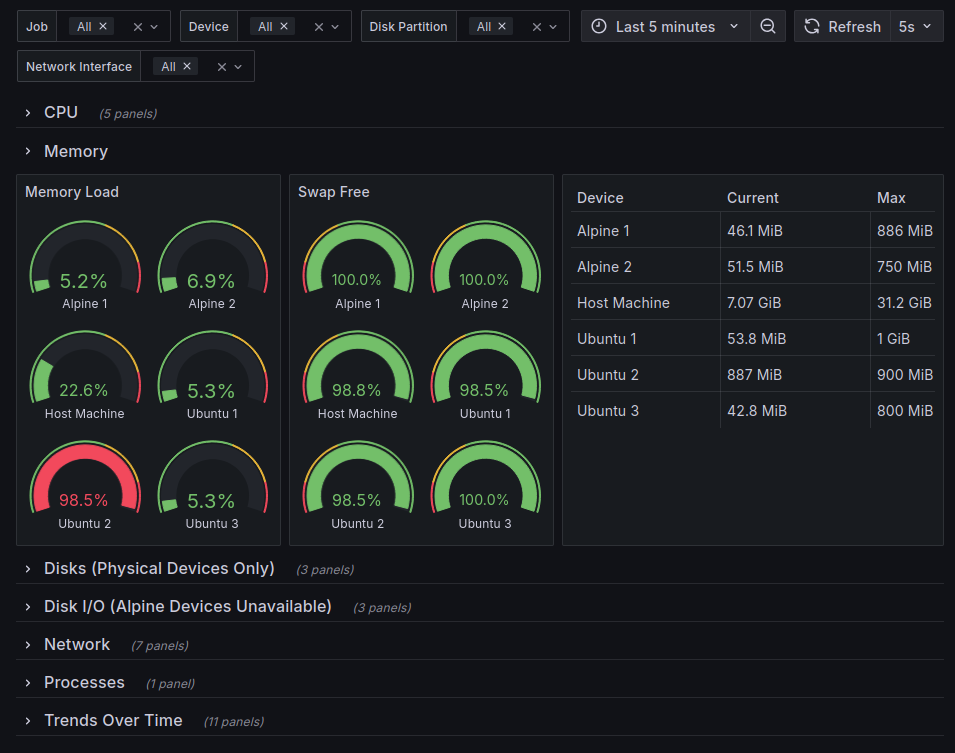
\includegraphics[width=\textwidth]{Imagens/chap04/dashboard/home.png}
\caption{Dashboard - Visão Geral.}
\label{fig:dashboard-home}
\end{figure}

{\color{red}
A Figura \ref{fig:dashboard-home} apresenta a visão geral do dashboard, desenvolvido para fornecer uma representação imediata e concisa do estado de saturação do sistema, permitindo ao usuário identificar rapidamente sinais de saturação elevada. Na parte superior, encontram-se os botões que possibilitam a interação do usuário com os dados. Do canto superior esquerdo até o centro estão as \verb|Grafana Variables|, listadas na Tabela \ref{tab:grafana-variables}, que funcionam como filtros seletivos. Do centro até o canto superior direito, estão localizados os seletores de janelamento histórico e frequência de atualização do dashboard.

O dashboard é organizado em seções horizontais que funcionam como um \foreign{dropdown}, segmentando as informações por categoria de métrica. No exemplo mostrado na Figura \ref{fig:dashboard-home}, a seção \myenquote{Memory} está expandida, exibindo gráficos e visualizações relacionados às métricas de memória coletadas. Esta mesma lógica aplica-se às demais seções, com exceção da seção \myenquote{Trends Over Time}.

Na seção \myenquote{Trends Over Time}, são exibidos gráficos de séries temporais para análise de dados históricos. Diferentemente das outras seções, aqui são apresentadas visualizações de todas as métricas coletadas. Essa ampliação do escopo permite que o usuário realize correlações entre as métricas, facilitando a investigação de problemas, como pode ser observado na Figura \ref{fig:dashboard-timeseries}.

\begin{figure}[H]
\centering
\color{red}
\setlength{\abovecaptionskip}{-20pt}
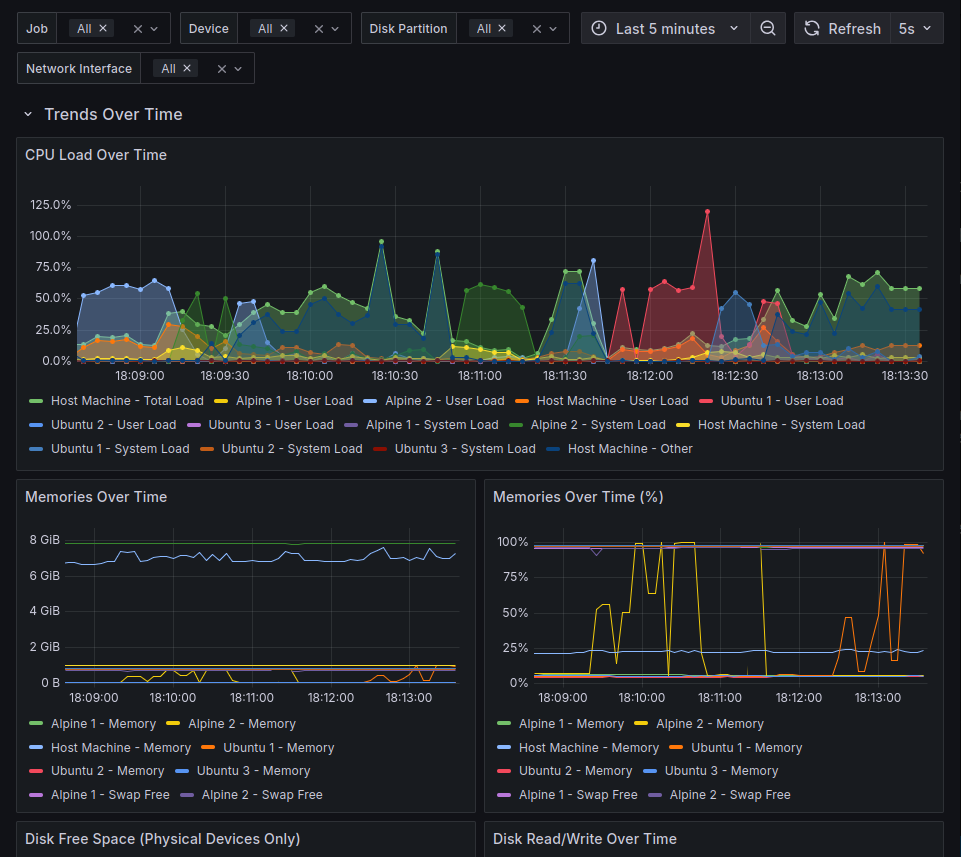
\includegraphics[width=\textwidth]{Imagens/chap04/dashboard/trends_over_time.png}
\caption{Séries Temporais.}
\label{fig:dashboard-timeseries}
\end{figure}

Na seção de CPU, ilustrada na Figura \ref{fig:dashboard-cpu}, 
têm-se gráficos de carga de usuário, carga de sistema, aguardo por I/O, carga total e cargas diversas, específicas de cada dispositivo. No entanto, como apresentado na Tabela \ref{tab:metricas-selecionadas}, algumas métricas não estão presentes em todos os dispositivos, como é o caso da métrica de aguardo por I/O, que não é coletada nos dispositivos virtuais.

Uma observação relevante é que, apesar da métrica de tempo ocioso estar disponível, para contêineres ela sempre apresenta o valor zero, em função da forma como o cgroup gerencia os recursos, impedindo assim o cálculo das métrica de carga total e cargas diversas, que dependem direta e indiretamente do tempo ocioso, respectivamente.

\begin{figure}[H]
\centering
\color{red}
\setlength{\abovecaptionskip}{-20pt}
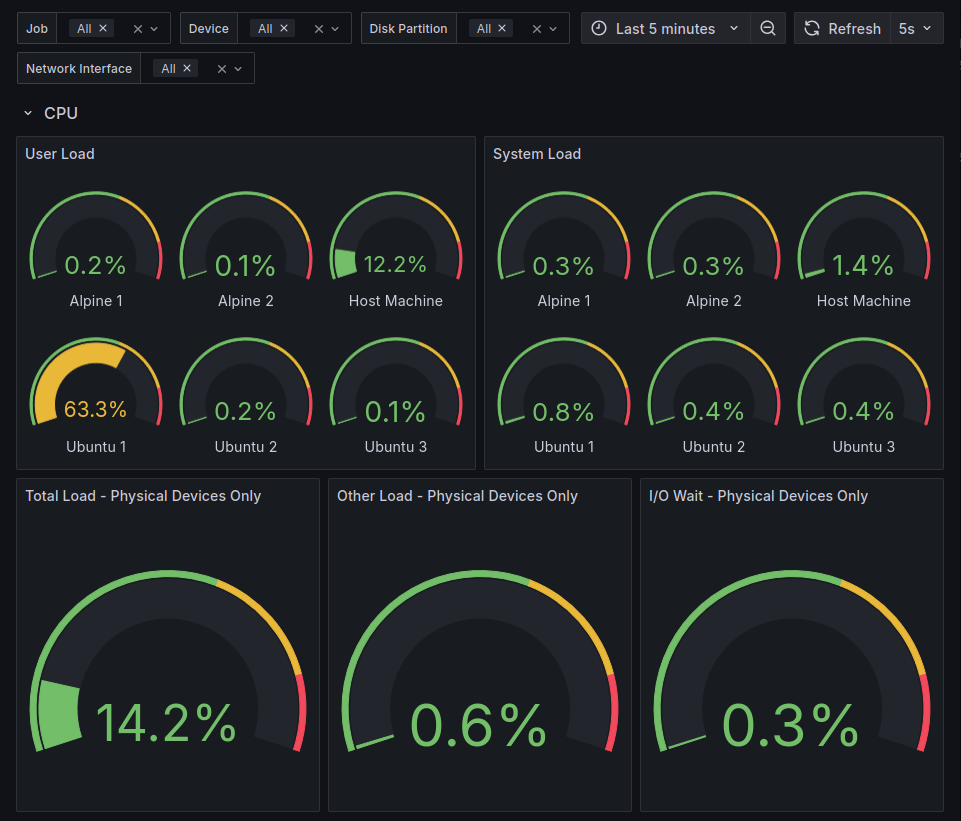
\includegraphics[width=\textwidth]{Imagens/chap04/dashboard/cpu.png}
\caption{Seção de CPU.}
\label{fig:dashboard-cpu}
\end{figure}

Na seção de memórias (ilustrada na Figura \ref{fig:dashboard-memory}), são apresentados gráficos de uso da memória RAM e memória swap disponível, enquanto na seção de Disco I/O (Figura \ref{fig:dashboard-diskio}), encontram-se gráficos de operações de leitura e escrita em disco. Destaca-se que nesta subseção observa-se a indisponibilidade de dados provenientes dos dispositivos Alpine. Isso ocorre devido a uma incompatibilidade entre a definição geral do \verb|inputs.cgroups| do Telegraf e a estrutura de cgroups do Alpine, o que provoca um erro de \foreign{parse} durante a leitura das métricas. Embora uma possível solução seja a criação de um arquivo de configuração específico para o Alpine, decidiu-se não implementá-la. Para fins ilustrativos, foi aplicado o filtro \verb|Device = Host Machine|, que seleciona o dispositivo físico.

\begin{figure}[H]
\centering
\color{red}
\setlength{\abovecaptionskip}{-20pt}
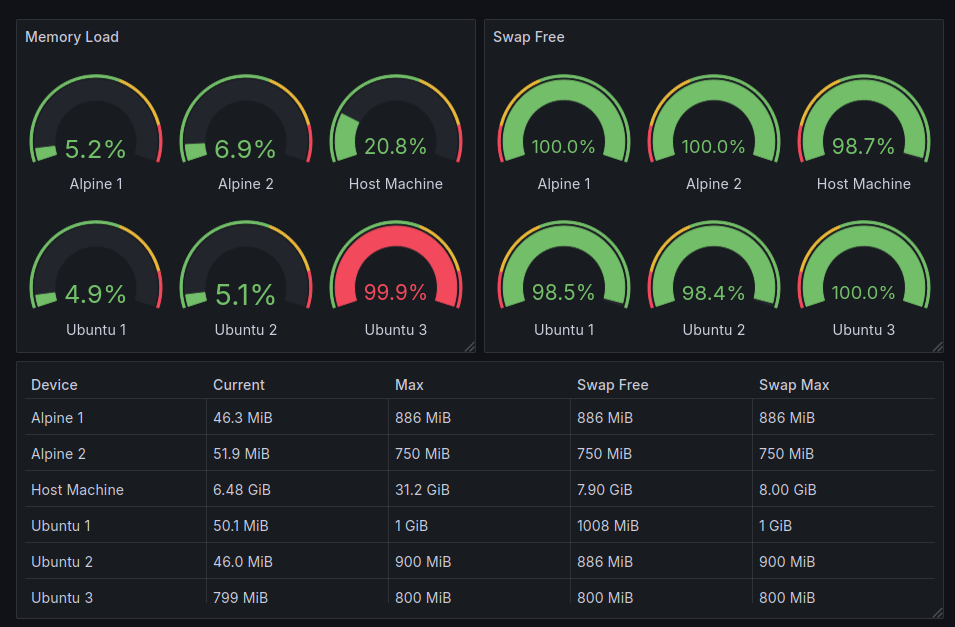
\includegraphics[width=\textwidth]{Imagens/chap04/dashboard/memory.png}
\caption{Seção de Memórias.}
\label{fig:dashboard-memory}
\end{figure}

\vspace{1cm}

\begin{figure}[H]
\centering
\color{red}
\setlength{\abovecaptionskip}{-20pt}
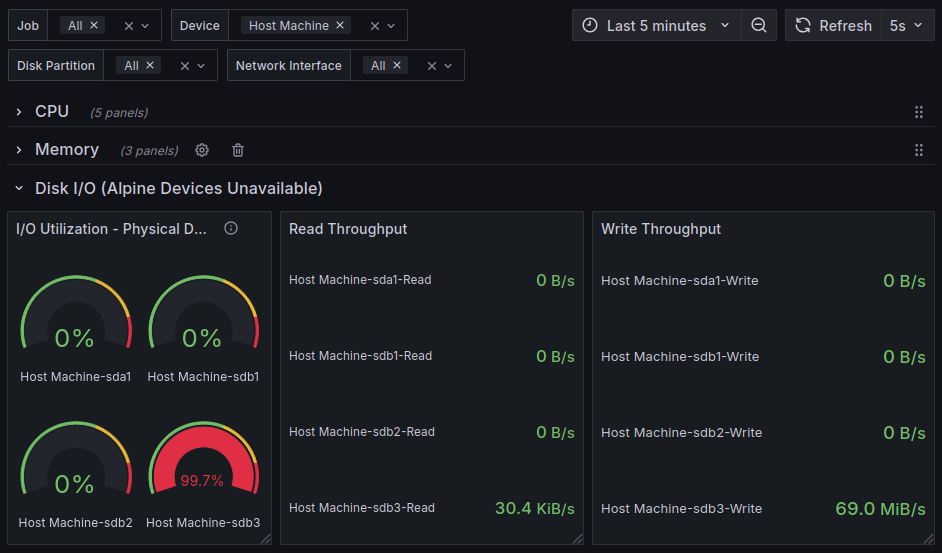
\includegraphics[width=\textwidth]{Imagens/chap04/dashboard/diskio.png}
\caption{Seção de Disco I/O.}
\label{fig:dashboard-diskio}
\end{figure}

Por conta das particularidades das métricas de disco --- como discrepâncias em disponibilidade, optou-se por separar métricas de disco em duas seções: as de leitura e escrita das métricas, apresentadas anteriormente, e as de espaço livre e utilizado em disco, além da quantidade de INODES livres, são apresentadas na seção de Disco (Figura \ref{fig:dashboard-disk}). 

\begin{figure}[H]
\centering
\color{red}
\setlength{\abovecaptionskip}{-20pt}
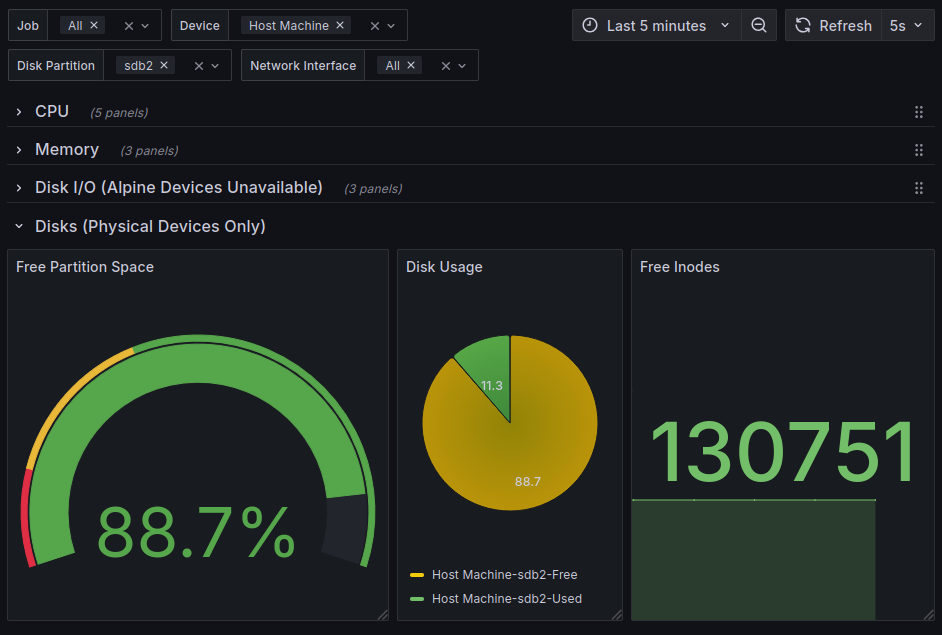
\includegraphics[width=\textwidth]{Imagens/chap04/dashboard/disk.png}
\caption{Seção de Disco.}
\label{fig:dashboard-disk}
\end{figure}

Uma observação importante, embora pouco intuitiva, refere-se à métrica de espaço total em disco. Embora esteja disponível, essa métrica não é a mais adequada para os cálculos dos gráficos. Para determinar o espaço total utilizado, conforme explicitado em nota na documentação do plugin \verb|inputs.disk| \citep{inputsdisk2025}, utiliza-se a soma dos valores de espaço livre e utilizado, descartando-se o valor da métrica de espaço total. Isso ocorre porque a métrica de espaço total reportada pelos sistemas de arquivos pode incluir blocos reservados para o superusuário (\foreign{root}) e outras finalidades do sistema, que não estão disponíveis para usuários comuns, enquanto a soma \myenquote{livre + utilizado} representa de forma mais fiel o espaço efetivamente utilizável.

Para validar a precisão dos dados, realizou-se a comparação entre os valores de espaço livre e utilizado coletados pelo Telegraf e os valores fornecidos pelo comando \verb|df -h| do Linux, uma das ferramentas mais utilizadas para essa finalidade. Os resultados indicaram que os valores obtidos pelo Telegraf apresentaram uma margem de erro inferior a 1\% quando comparados aos valores fornecidos pelo comando \verb|df -h|, provando a confiabilidade das métricas coletadas.

\begin{figure}[H]
\centering
\color{red}
\setlength{\abovecaptionskip}{-20pt}
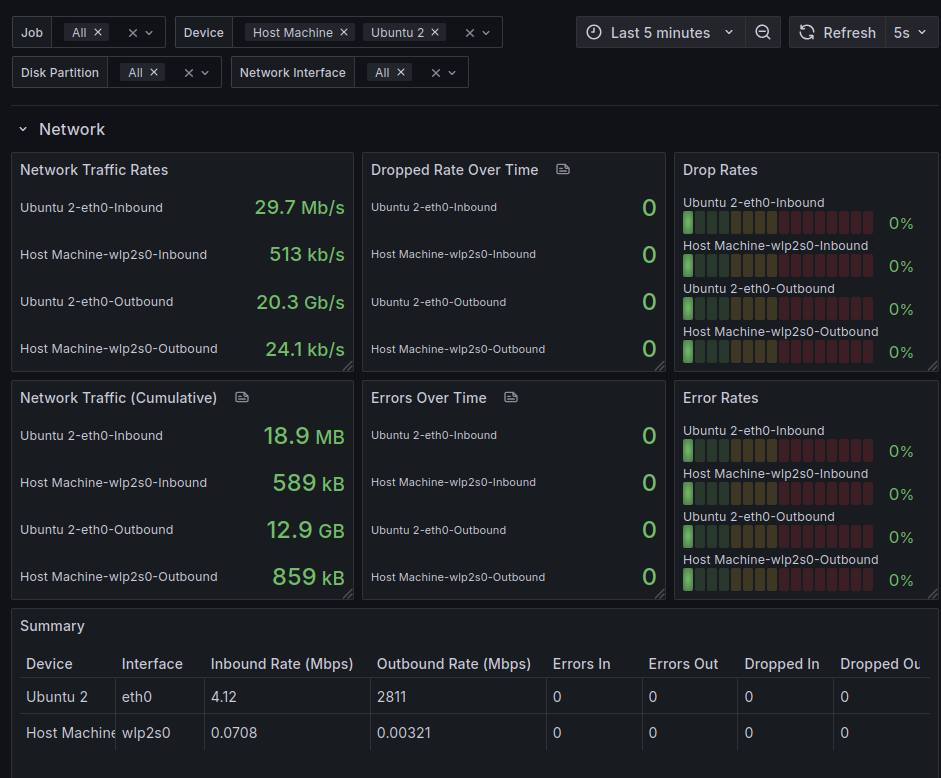
\includegraphics[width=\textwidth]{Imagens/chap04/dashboard/network.png}
\caption{Seção de Rede.}
\label{fig:dashboard-network}
\end{figure}

A Figura \ref{fig:dashboard-network} apresenta a seção de Rede, na qual, mais uma vez para fins ilustrativos, aplicou-se o filtro de dispositivos, nesta ocasião selecionando dos dispositivos \myenquote{Host Machine} e \myenquote{Ubuntu 2}. Essa seção exibe valores instantâneos e acumulativos de tráfego de rede, bem como as quantidades de pacotes descartados ou com erros.

A ausência de dados sobre pacotes descartados ou com erros nos dispositivos virtuais está relacionada à camada de coleta dessas métricas. Tentativas de utilização das ferramentas de \foreign{chaos-engineering} Pumba e ChaosBlade, bem como manipulações diretas no \verb|iptables| para geração de tráfego de rede, mostraram-se inadequadas para este estudo.

Por debaixo dos panos, ferramentas de \foreign{chaos testing} utilizam para testes de rede o módulo \verb|netem| do sistema \verb|tc| do Linux. Esse sistema opera na camada de controle de tráfego (\verb|qdisc|), enquanto o \foreign{plugin} \verb|inputs.net| do Telegraf opera a partir da leitura do \verb|procfs/net/dev|, que se encontra na camada de interface de rede. Por tanto, por estarem em camadas distintas, o Telegraf é incapaz de captar as informações de pacotes descartados ou com erros contabilizados pelo sistema.

\begin{figure}[H]
\centering
\color{red}
\setlength{\abovecaptionskip}{-20pt}
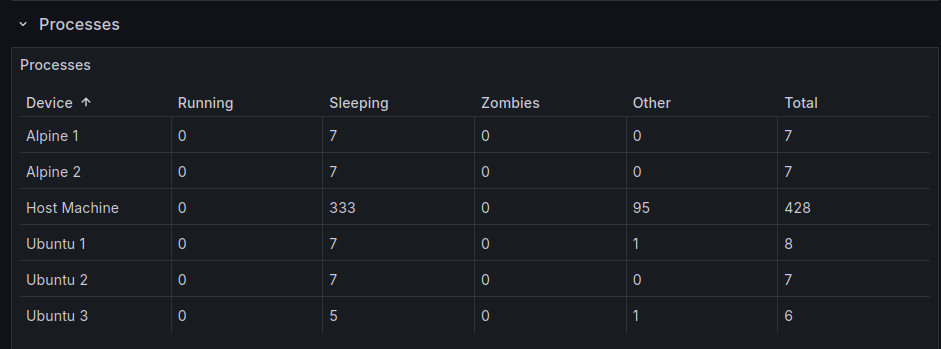
\includegraphics[width=\textwidth]{Imagens/chap04/dashboard/processes.png}
\caption{Seção de Processos.}
\label{fig:dashboard-processes}
\end{figure}

Finalmente, a Figura \ref{fig:dashboard-processes} exibe uma tabela com as quantidades dos processos selecionados, conforme especificado na Tabela \ref{tab:metricas-selecionadas} da Seção \ref{section:DiscussaoMetricas} do capítulo anterior.

Retornando à seção de séries temporais, destacam-se dois gráficos específicos: o uso de CPU e o uso de RAM. Na Figura \ref{fig:dashboard-cpu144}, observa-se que a carga de usuário da CPU no dispositivo virtual 3 ultrapassou 100\%. Embora possa parecer contraditório, visto que na Tabela \ref{tab:EspecificaçõesDispositivosVirtuais} foi estabelecido um limite máximo de utilização de 70\% para um único núcleo de CPU, esse fenômeno decorre das limitações do Docker na imposição de limites de CPU.

Assim, apesar da limitação, a figura evidencia que o contêiner pode apresentar picos de utilização superiores a 100\%, ou seja, utilizar mais de um núcleo de CPU. No caso específico apresentado, o valor de 144\% indica que o contêiner utilizou o equivalente a 1,44 núcleos de CPU.

Por fim, na figura \ref{fig:roundrobin}, observa-se a sequência rotativa de execução dos testes de saturação, conforme detalhado na Seção \ref{subsection:TestesSaturacao}. Essa rotação é evidenciada pelos picos alternados de utilização de memória entre os dispositivos virtuais, demonstrando que os testes foram executados de forma síncrona e sequencial, conforme implementado.

Após o desemvolvimento do \foreign{dashboard}, o mesmo foi exportado em formato JSON e versionado no repositório do projeto \citep{vitorcossetti2025}, na pasta \verb|configs/grafana/dashboards|. A configuração do Grafana foi ajustada para carregá-lo automaticamente via volume Docker, conforme detalhado no Capítulo \ref{chap3}.

\begin{figure}[H]
\centering
\color{red}
\setlength{\abovecaptionskip}{-20pt}
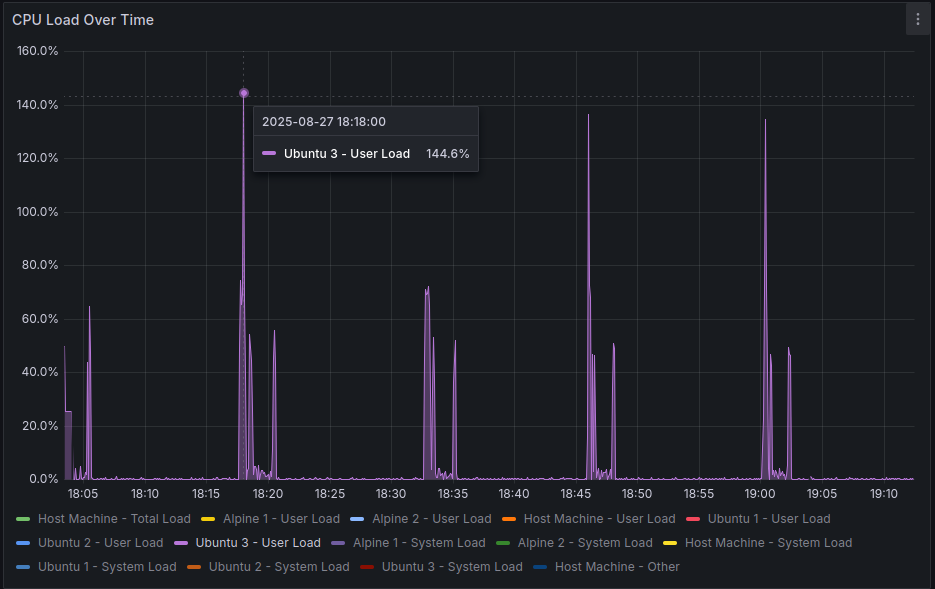
\includegraphics[width=\textwidth]{Imagens/chap04/dashboard/cpu144.png}
\caption{Pico de 144\% de carga de usuário para CPU.}
\label{fig:dashboard-cpu144}
\end{figure}

\begin{figure}[H]
\centering
\color{red}
\setlength{\abovecaptionskip}{-20pt}
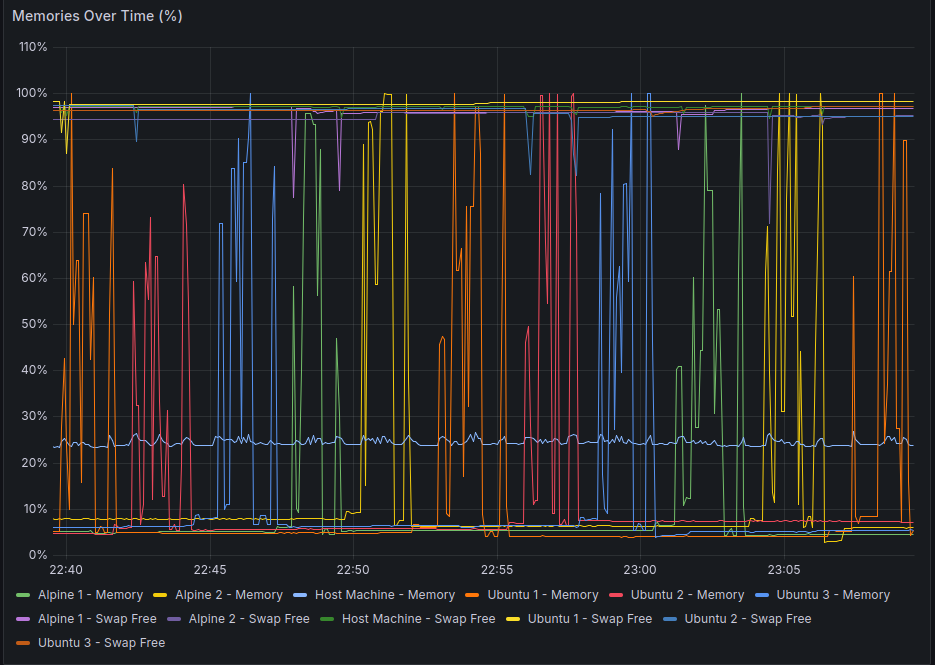
\includegraphics[width=\textwidth]{Imagens/chap04/dashboard/round_robin_sequence.png}
\caption{Sequência rotativa de execução de carga.}
\label{fig:roundrobin}
\end{figure}













\section{Alertas e Notificações}
\label{section:Alertas}

Para o sistema de alertas, inicialmente foram exploradas as funcionalidades nativas do Grafana, que permitem a criação de alertas diretamente na interface web. Essa abordagem inicial foi adotada devido à sua simplicidade e integração direta com os gráficos do dashboard, facilitando a associação visual entre os dados monitorados e os alertas correspondentes.

Como canais de comunicação, foram configurados o envio de e-mails e notificações por aplicativo de mensagens. A configuração do canal de e-mail utilizou o servidor SMTP do Gmail, enquanto a integração com o aplicativo foi realizada por meio da criação de um bot específico para esse propósito. Entretanto, a integração com o aplicativo apresentou desafios técnicos que resultaram em erros, inviabilizando seu uso para notificações, restando somente o canal de e-mail funcional.

Além dos pontos de contato e canais, foram definidas políticas de notificação e regras de alerta baseadas em limiares específicos para as métricas monitoradas. Essas regras foram configuradas para disparar notificações quando determinados parâmetros ultrapassassem valores críticos durante um período estabelecido.

No entanto, essa abordagem apresentou uma limitação crítica. O Grafana, em sua configuração padrão, utiliza o banco de dados SQLite, o que implica que o gerenciamento de alertas, notificações, estados, \foreign{logging} e outros serviços sujeitos a alta frequência de escrita são armazenados em um banco de dados não otimizado para grandes volumes de operações concorrentes. Essa limitação tornou-se evidente quando o sistema passou a apresentar falhas constantes devido a erros de \foreign{database lock}, como \foreign{max-retries-reached}.

Diante dessa criticidade, optou-se pela migração do banco de dados do Grafana para PostgreSQL. Essa migração foi facilitada pela abordagem de IaC adotada, bem como pelo fato de o armazenamento persistente dos dados coletados ficar sob responsabilidade do Prometheus, que já utilizava o TSDB. A migração foi realizada de forma simples, adicionando um contêiner baseado na imagem oficial do PostgreSQL e configurando os parâmetros do Grafana para integração com o novo banco e uso de volumes Docker. Após a migração, o sistema apresentou melhora significativa na estabilidade e no desempenho, eliminando os erros de \foreign{database lock} e permitindo uma gestão mais eficiente dos alertas e notificações.

Entretanto, essa migração evidenciou uma questão arquitetural. A solução inicialmente adotada, embora funcional, introduzia complexidade adicional ao requerer a manutenção de dois bancos de dados distintos: o TSDB do Prometheus e o PostgreSQL do Grafana. Essa complexidade poderia ser evitada com a adoção do Alertmanager, ferramenta nativa do Prometheus para gerenciamento de alertas. O Alertmanager é projetado especificamente para lidar com alertas gerados pelo Prometheus, oferecendo funcionalidades avançadas de roteamento, agrupamento e silenciamento de alertas, além de suporte nativo a múltiplos canais de notificação.

Assim, decidiu-se migrar o sistema de alertas para o Alertmanager, integrando-o diretamente com o Prometheus. A implementação dessa mudança enfrentou alguns desafios, uma vez que o contêiner do Alertmanager, baseado na imagem oficial, apresentava dificuldades na leitura dos arquivos de configuração do projeto. Essas limitações foram superadas mediante a criação de um novo contêiner Alpine customizado, configurado com o Alertmanager e ferramentas essenciais como \verb|curl| e \verb|gettext|, além de um script para automatizar a leitura e validação dos arquivos de configuração em tempo de execução. Apesar da complexidade adicional introduzida para contornar as limitações da imagem oficial, essa solução permitiu uma integração eficiente do Alertmanager com o restante da arquitetura.

Após a integração do Alertmanager, todas as configurações previamente realizadas no Grafana foram migradas sem dificuldades, considerando que ambas as plataformas utilizam arquivos YAML para configuração. Em seguida, realizou-se o \foreign{rollback} do banco de dados do Grafana para SQLite, visando simplificar a arquitetura e reduzir o custo computacional do sistema. Embora com frequência significativamente menor, eventuais falhas de \foreign{database lock} foram novamente detectadas, corroborando a recomendação da literatura contra a utilização do SQLite em cenários de alto volume de escrita concorrente, o que tornou necessário manter o PostgreSQL como SGDB\abbrev{SGDB}{Sistema Gerenciador de Banco de Dados} do Grafana.

Pode-se questionar por quê não retornar ao uso do Grafana como gerenciador de alertas, considerando que a manutenção de um banco de dados adicional mostrou-se inevitável e a adição do Alertmanager introduziu complexidade extra. A resposta reside no fato de que, para cada alerta criado no Grafana, uma consulta PromQL percorre todo o fluxo descrito na Seção \ref{section:Dashboard}, podendo aumentar significativamente o custo computacional do sistema, especialmente em ambientes de alta escalabilidade com múltiplos alertas e gráficos. Por outro lado, no Alertmanager, os alertas são gerados diretamente pelo Prometheus, eliminando a necessidade de consultas adicionais e reduzindo o impacto no desempenho do sistema. Portanto, a otimização na execução das regras de alertas justifica o custo do contêiner adicional do Alertmanager.

\begin{figure}[H]
\centering
\setlength{\abovecaptionskip}{-20pt}
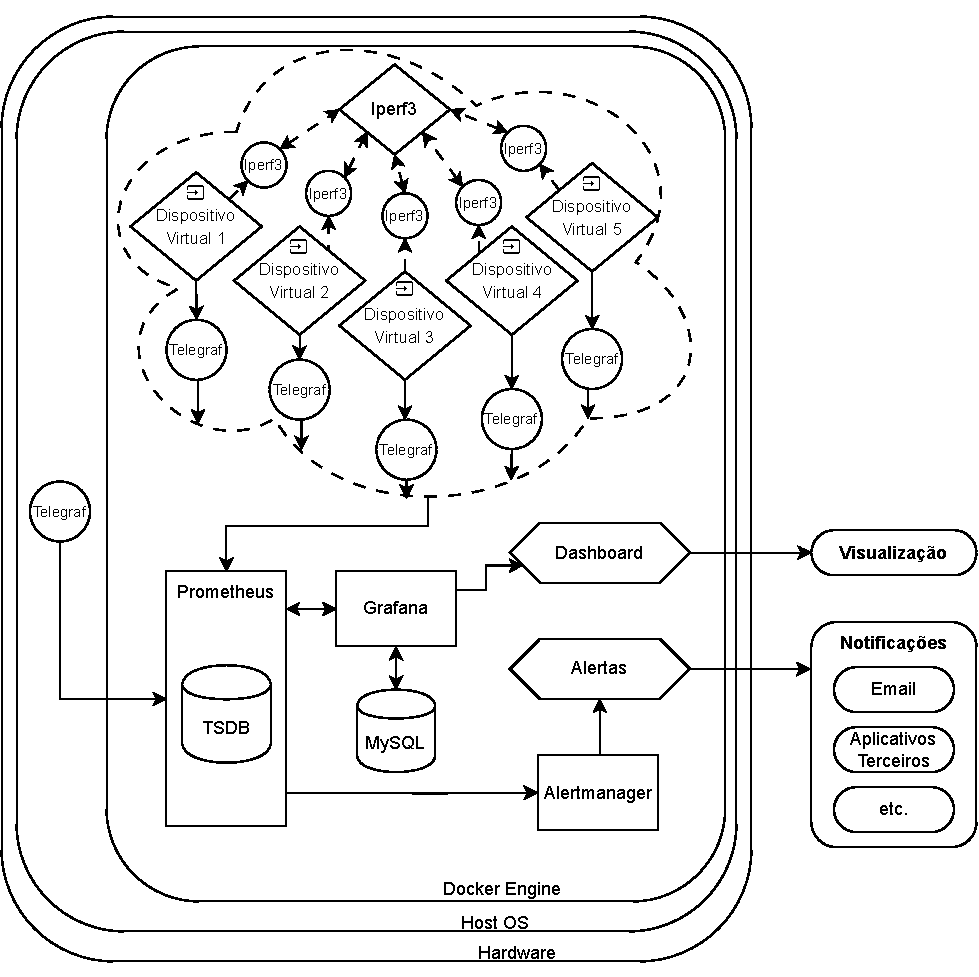
\includegraphics[width=\textwidth]{Imagens/chap04/by-blocks/alerts_diagram.pdf}
\caption{Notificações e Diagrama Final.}
\label{fig:DiagramaAlertas}
\end{figure}

Um exemplo de alerta implementado é o alta carga de escrita/leitura em disco, cuja regra é apresentada no Código Fonte \ref{lst:HighDiskIOAlert}:

\newpage

\begin{lstlisting}[caption={Alerta para alta carga de escrita/leitura em disco}, label={lst:HighDiskIOAlert}]
groups:
  - name: disk_alerts
    interval: 180s
    rules:
      - alert: HighDiskIO
        expr: physical_diskio_io_util{job=~".*", alias=~".*", disk_partition=~".*"} >= 85
        for: 10m
        labels:
          severity: warning
          team: sre
        annotations:
          summary: "Disk I/O Load >= 85%"
          description: "Over the last 10 minutes, the disk i/o was above 85% on {{ $labels.alias }}-{{ $labels.disk_partition }}."
\end{lstlisting}

O código \ref{lst:HighDiskIOAlert} define um alerta agrupado em \verb|disk_alerts|, que é avaliado a cada 180 segundos. A regra do alerta, denominada \verb|HighDiskIO|, é disparada quando a métrica \verb|physical_diskio_io_util| atinge ou ultrapassa 85\% por um período de 10 minutos. O alerta é categorizado com o rótulo de severidade \verb|warning| e direcionado à equipe \myenquote{sre}. As anotações fornecem um resumo e uma descrição detalhada do alerta, incluindo informações dinâmicas sobre o dispositivo e a partição afetados.

Ou seja, numa janela de 10 minutos, coletam-se amostras a cada 180 segundos e, se todas as amostras indicarem que a métrica de utilização de I/O de disco está igual ou acima de 85\%, o alerta será disparado.

A Figura \ref{fig:alert_prometheus} apresenta o alerta em execução no Prometheus, enquanto a Figura \ref{fig:alert_alertmanager} ilustra dois alertas disparando no Alertmanager. Já a Figura \ref{fig:alert_email} exibe um exemplo de alerta recebido via e-mail. 
\begin{figure}[H]
\centering
\color{red}
\setlength{\abovecaptionskip}{-20pt}
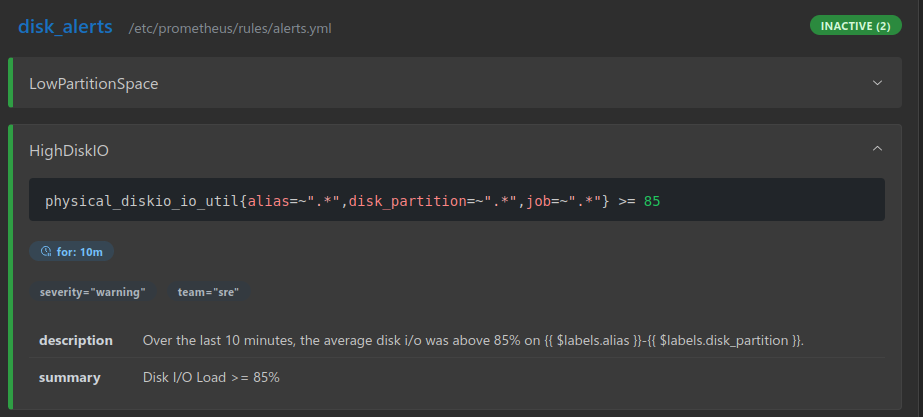
\includegraphics[width=\textwidth]{Imagens/chap04/alerts/alert_prometheus.png}
\caption{Alerta no Prometheus.}
\label{fig:alert_prometheus}
\end{figure}

\begin{figure}[H]
\centering
\color{red}
\setlength{\abovecaptionskip}{-20pt}
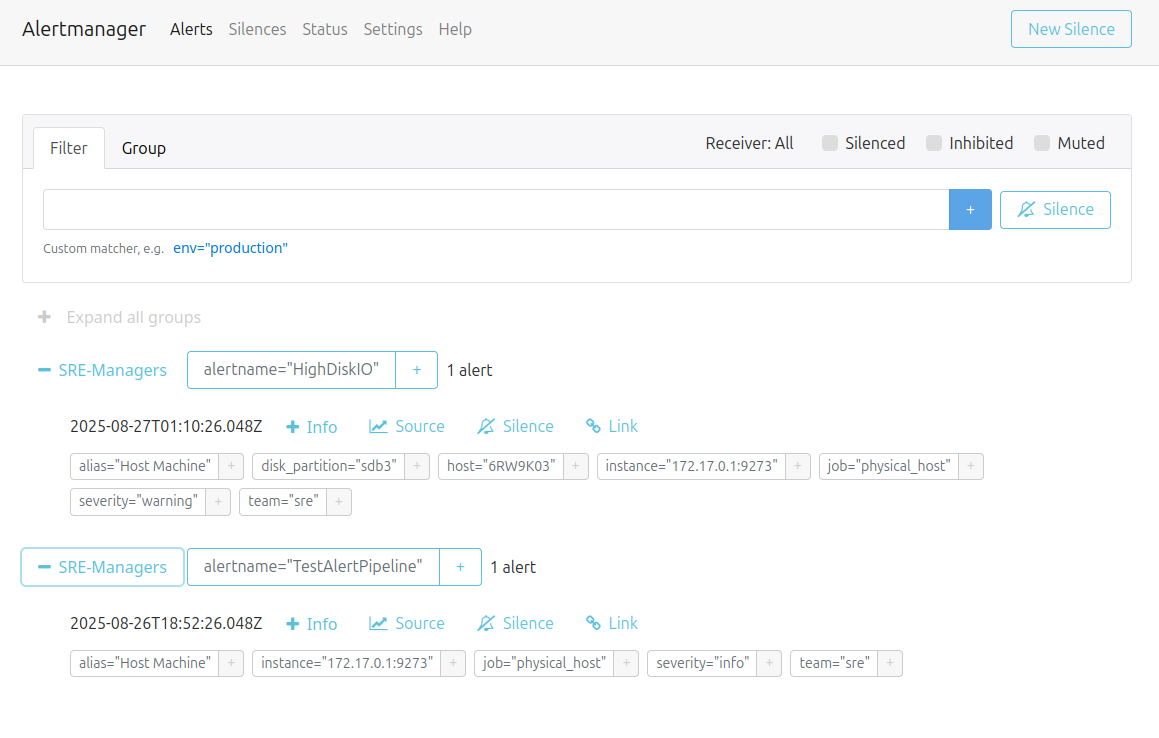
\includegraphics[width=\textwidth]{Imagens/chap04/alerts/alert_alertmanager.png}
\caption{Alertas no Alertmanager.}
\label{fig:alert_alertmanager}
\end{figure}

\begin{figure}[H]
\centering
\color{red}
\setlength{\abovecaptionskip}{-20pt}
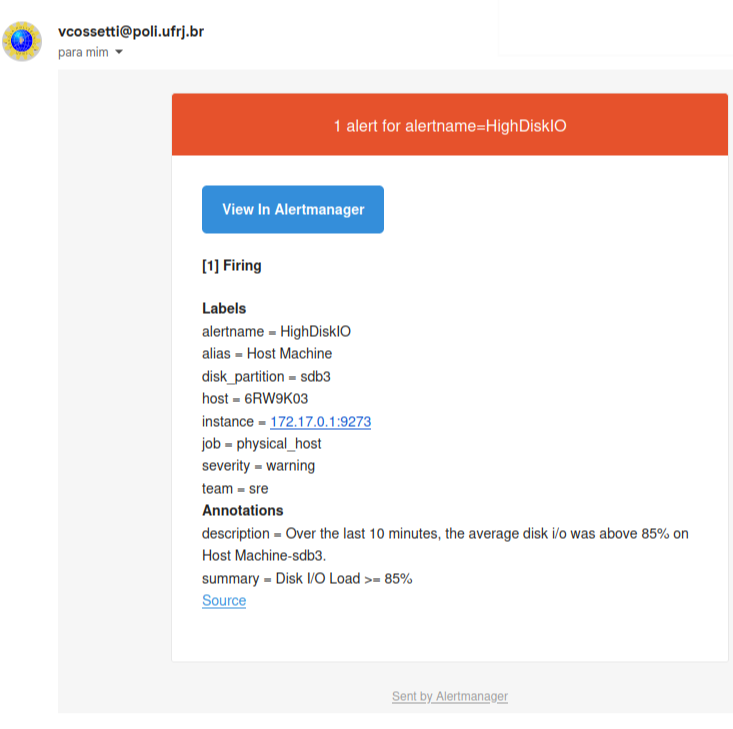
\includegraphics[width=\textwidth]{Imagens/chap04/alerts/alert_email.png}
\caption{Exemplo de alerta via email.}
\label{fig:alert_email}
\end{figure}







}

\section{Caso de Uso}
\label{section:CasosDeUso}

Um caso de uso para este projeto é o monitoramento da saturação dos equipamentos do próprio autor. Com o dashboard e notificações de alertas desenvolvidos nestre trabalho, foi possível identificar causadores de travamentos, como picos de \myenquote{Aguardo de I/O} da CPU e \myenquote{Utilização I/O} de disco quando executando os testes de saturação dos contêineres de forma assíncrona, o que motivou para a mudança para a execução síncrona dos testes, conforme detalhado em \ref{subsection:TestesSaturacao}.

{\color{red}
A Figura \ref{fig:StackFinal} apresenta a arquitetura final do sistema de monitoramento, incluindo todos os componentes, implementações e integrações descritas ao longo deste trabalho. Na Seção \ref{subsection:VersõesIniciais}, detalhou-se a evolução da arquitetura desde suas versões iniciais até a configuração com Docker, Prometheus e Grafana. Na Subseção \ref{subsection:DispositivosVirtuais}, descreveu-se a implementação dos dispositivos virtuais por meio de contêineres Docker. Na Subseção \ref{subsection:Agentes}, abordou-se a configuração dos agentes de coleta de métricas utilizando o Telegraf. Em \ref{subsection:TestesSaturacao}, detalhou-se a metodologia de testes de saturação aplicada aos dispositivos virtuais. Por fim, na Seção \ref{section:Alertas} foi detalhada a implementação do sistema de alertas, a necessidade da adoção de um SGDB capaz de operar com múltiplas tarefas concorrentes, como o PostgreSQL, e a utilização de notificações por meio do Alertmanager.}
\begin{figure}[H]
\centering
\setlength{\abovecaptionskip}{-20pt}
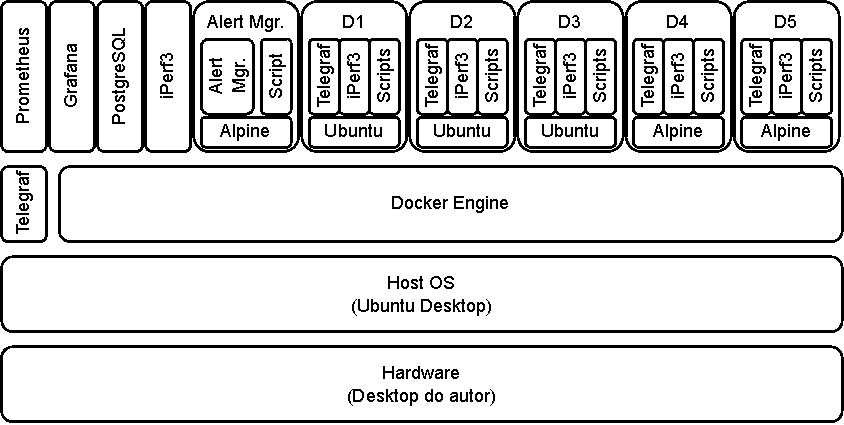
\includegraphics[width=\textwidth]{Imagens/chap04/final_stack.pdf}
\caption{\foreign{Stack} final.}
\label{fig:StackFinal}
\end{figure}


